\documentclass{article}
\usepackage[utf8]{inputenc}
\usepackage{float}
\usepackage{graphicx}
\usepackage{xcolor, soul}
\usepackage[english]{babel}
\usepackage[margin=1.7in]{geometry}
\bibliographystyle{unsrt}
\usepackage{hyperref}
\usepackage{amsmath}
\usepackage{amssymb}
\usepackage{subcaption}
\usepackage{mathtools}
\usepackage{tabularx,ragged2e,booktabs,caption,sidecap,subcaption,graphicx,tikz}

\begin{document}
\begin{titlepage}
	
	
	\title{Project 2 \\ Course 02445 \\ Project in Statistical evaluation of \\ artificial intelligence }
	\author{Rasmus J. P. s164564 \\ Nikolaj S. P. s183930}
	\date{January 2020}
	\maketitle
	
\subsection*{Summary}
In most industries learning from data is second nature but as data collection become very expensive and time consuming, deciding what to collect and how to collect it naturally follows. That is a data scientist's job to answer and in this report we examine two different techniques of measuring bio-available phosphorous in soil and analyze both techniques using a linear- and a non-linear model.\\ We conclude by analyzing data that bio-available phosphorous does have an influence on the yield of Barley but only up to a certain amount whereas afterwards increasing phosphorous in soil does not have a significant effect on the yield of barley. We conclude that the two measuring techniques were significantly different and make recommendation towards the more expensive technique DGT and that the yield be estimated by a non-linear model.
	
\end{titlepage}


\section{Introduction}
Crops need nutrients and if the levels of certain nutrients is too low the yield will be affected. Measuring the bio-available phosphorous BAP in soil is an important task for farmers in order to provide his or hers crops with sufficient amounts of nutrients. We know that the BAP is an important nutrient for plants but how big exactly is this influence of BAP to the yield of barley if it's there at all? That is the first aim of this report - to analyze and determine whether there is a significant influence from BAP on the yield and try and determine a model that best describes this proposed effect. We analyze the models and evaluate them on their fit to actual data using Leave-one-out cross validation LOOCV. \\ A new and more expensive measurement technique "DGT" is proposed to be better than the older "Olsen P" technique. Analyzing these two techniques is the second aim for this report and to determine if there's a significant difference between the two in order to make a well-informed and guided recommendation for farmers.We will use a paired Student's t-Test to compare the squared error values from the LOOCV algorithm.




\section{Data}
An experiment was performed on nine different fields spread across Denmark and Norway and each field partitioned into 4 plots. The yield of barley was measured and soil samples were analyzed by two measuring techniques, "DGT" and "Olsen P".
The data contains 4 variables, three continuous and 1 categorical. The continuous variables are \textit{yield ($hkg/ha$), DGT ($\mu/L$), Olsen P ($mg/100g$)} and the categorical is a unique identification number for each of the nine fields.
Observations were collected one from each of the plots in the nine fields resulting in 36 observation of 4 variables.
We decided to impute two missing data points with the mean of other plots from the same field.
Our reasoning behind imputing the data was firstly, the fields do not have a high variance of yield between the plots, which means replacing the missing values with the mean would likely not be too far off from the real values.
Secondly, field 11 has important observation with the lowest measurements of BAP and removing it might heavily impact our models. See figure \ref{fig:loc} for a boxplot from each field.
 
\begin{figure}[H]
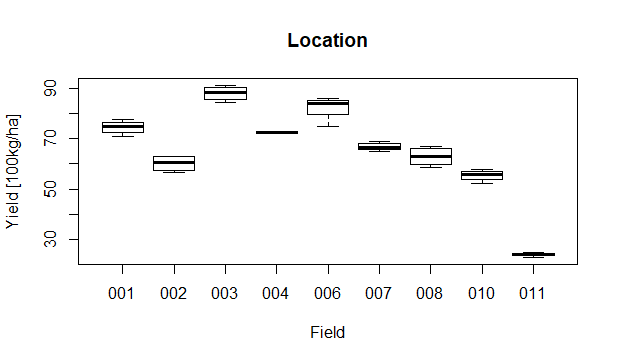
\includegraphics[width=\linewidth]{locationYield.png}
\caption{"Boxplot of yield for each field. We can see the variance within a field is relatively low, and location looks to have influence on yield"}
\label{fig:loc}
\end{figure}


\section{Methods and Analysis}
We start our analysis by assuming a linear correlation between response (yield), and our term (BAP measured with both Olsen P and DGT techniques). The resulting models are then evaluated on how well they fit to data via analysis of variance ANOVA. \\ A non-linear model namely Michaelis-Menten model MM, see equation (1), is used and just as before we evaluate the fit of this new model.
\begin{equation}
y = \frac{\alpha \cdot x}{\beta + x}
\end{equation}
For now we will focus on comparing the two measuring techniques using the non-linear model. \\ Using R's nls() function we fit the Michaelis-Mente models to data and record the resulting parameters and their p-values taking extra care that the $\beta$ parameter is a number non-zero i.e. a beta of zero would result in the model $y = \alpha$ removing BAP as a variable and making it non-significant. 

Examining the fit of the four different models we first take a look at the resulting regression lines, we plot the lines together with the actual yield data, see figure \ref{fig:linearnonlinear}.
\begin{figure}[H]
	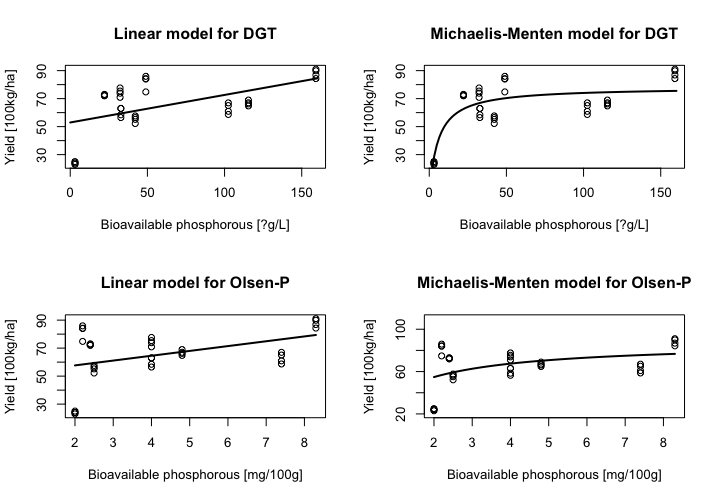
\includegraphics[width=\linewidth]{linearnonlinear.png}
	\caption{"Linear regression models to the left and non-linear \textit{Michaelis Mente models"} on the right. "}
	\label{fig:linearnonlinear}
\end{figure}


It can be hard to discern which lines best explain the correlation by just looking at plots, and in fact a few of the residual standard errors also seem quite equal, but looking at the model errors in a quantile-quantile plot we see that the errors diverge from normality in the linear model, see figure \ref{fig:qqplot}. The non-linear model from the second row shows little deviation from normality with only one apparent outlier within the confidence envelope
\begin{figure}[H]
	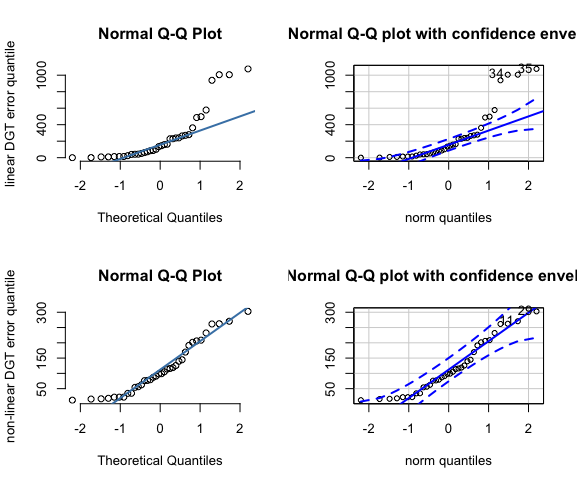
\includegraphics[width=\linewidth]{qqplot.png}
	\caption{"QQ-plot for DGT technique, top row is from the linear model and bottom row from the \textit{Michaelis Mente model}", second column show a 0.95 confidence envelope}
	\label{fig:qqplot}
\end{figure}

For a  respective p-values we see a sharp difference in the confidence of the coefficients. See table \ref{tab:p-values} for the standard squared error and respective p-values for each model.


\subsection{Accuracy validation and testing}
To maximize the accuracy of our estimated parameters we perform leave-one-out cross validation LOOCV and save the squared error of each fold for all four  models i.e. a non-linear- and a linear model where term is the "Olsen P" and the same where it is "DGT". We then do a comparison of means with a paired two-sampled t-test.


\section{Results}
In table \ref{tab:p-values} we present our summed statistical analysis of variance for each separate model. The first thing we notice is that both of the standard linear models, the models fitted as: response ~ intercept+slope*term turn out to perform quite well with a Residual standard error RSE of $15.37$ for DGT technique and $16.55$ for the Olsen P. Looking at the two non-linear models the difference becomes more apparent with RSE values of $10.58$ for DGT and $16.33$ for Olsen P. 

\begin{table}\hspace{-2.1cm}
\begin{tabular}{lcccc}\toprule [1.5pt]
\textbf{Model}                & \multicolumn{1}{l}{\textbf{Linear DGT}} & \multicolumn{1}{l}{\textbf{Linear Olsen-P}} & \multicolumn{1}{l}{\textbf{Non-linear DGT}}  & \multicolumn{1}{l}{\textbf{Non-linear Olsen-P}}         \\ \midrule
\textbf{Std squared error} & 15.37        & 16.55             & 10.58             &    16.33           \\\midrule
\textbf{p-values}   & DGT = 0.000685       & Olsen-P = 0.0103      & \begin{tabular}[c]{@{}c@{}}Alpha = 2e-16\\ Beta = 0.0014\end{tabular} & \begin{tabular}[c]{@{}c@{}}Alpha = 1e-9\\ Beta = 0.0432\end{tabular}\\
\bottomrule[1.25pt]
\end{tabular}
\caption{Model summary for values of fit}
\label{tab:p-values}
\end{table}

Comparing each model's performance to one another in a paired t-test keeping folds identical i.e. leave-one-out, we arrive at the data in table \ref{tab:BAPcompare}. Notice at the bottom of the table that we cannot say whether the Michaelis-Mente non-linear model is better than the linear one when using the Olsen P measurement technique. The same goes for the difference DGT vs Olsen P both linear. Figure \ref{fig:modelCI} show a 0.95 confidence envelope for the parameters.

\begin{table}[H]
\begin{tabular}{lccc}\toprule[1.5pt]
\textbf{Paired t-test between:}                          & \multicolumn{1}{l}{\textbf{t-statistic}} & \multicolumn{1}{l}{\textbf{df}} & \multicolumn{1}{l}{\textbf{p-values}} \\\midrule
\textbf{Non-Linear DGT - Non-linear Olsen-P} & -2.694                                   & 35                              & 0.011                                 \\\midrule
\textbf{Non-Linear DGT - Linear Olsen-P}     & -2.481                                   & 35                              & 0.018                                 \\\midrule
\textbf{Non-Linear DGT - Linear DGT}         & -2.381                                   & 35                              & 0.023                                 \\\midrule
\textbf{Linear DGT - Linear Olsen-P}         & -1.874                                   & 35                              & 0.069                                 \\\midrule
\textbf{Linear DGT - Non-linear Olsen-P}     & -1.590                                   & 35                              & 0.12                                  \\\midrule
\textbf{Linear Olsen-P - Non-linear Olsen-P} & 0.3065                                   & 35                              & 0.76                      \\
\bottomrule[1.25pt]           
\end{tabular}
\caption{The table shows the result of comparing the 30 values of accuracy from each model in a paired t-test, the degrees of freedom and p-values.}
\label{tab:BAPcompare}
\end{table}


From table \ref{tab:p-values} we learned that the non-linear model with the DGT measuring technique had the lowest value of RSE. Our subsequent test, see table \ref{tab:BAPcompare} shows that this, lowest of all RSE scores, also is significantly different than all others. \\
With 35 observation per model it would be safe to assume a normal distribution and then lookup z-scores, but this will only result in even lower p-values for the ones that are already significant and even higher p-values for those that are not. Using the Student's t-statistics we effectively raises the requirements for significance.	



\begin{figure}[H]
	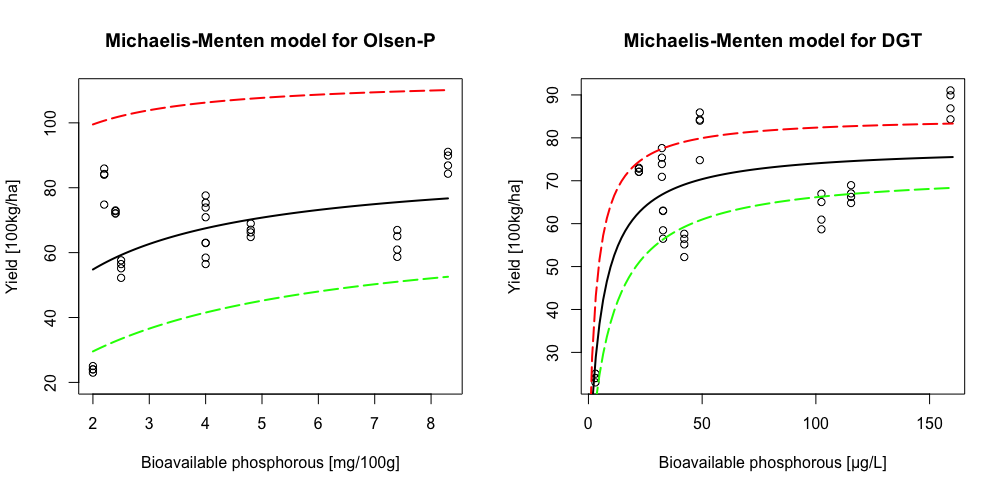
\includegraphics[width=\linewidth]{modelsEnv.png}
	\caption{Model with confidence interval}
	\label{fig:modelCI}
\end{figure}



\section{Discussion and Conclusion}

From our analysis we conclude that our investigation was well-founded, with a $\alpha = 0.95$ for the difference between using DGT- and Olsen P techniques in favor of the more expensive DGT. It  must also be noted that had we only done a linear regression model, we would not have come to the same conclusion. \\ All 4 models showed a 0.95 level of significant influence of bio-available phosphorous in the soil on the resulting yield of barley but only the non-linear DGT model had normally distributed residuals. 
We still discovered an outlier in the aforementioned model and considering the very small dataset for an industry of this magnitude we see potential in further developing model upon future data-collection.


\section{Appendix}
Public Github link for code and files: https://github.com/realnikolaj/02445

\end{document}